\documentclass[11pt,letterpaper]{article}

%\usepackage{fontspec}
%\usepackage[utf8]{inputenc}
\usepackage{textcomp,marvosym}
\usepackage{amsmath,amssymb}
\usepackage[normalem]{ulem}
\usepackage[left]{lineno}
\usepackage{changepage}
\usepackage{rotating}
\usepackage{color}
\usepackage{natbib}
\usepackage{setspace}
\usepackage{}
\usepackage{fancyhdr}
\usepackage{graphicx}
\usepackage{xspace}
\usepackage[hidelinks]{hyperref}
\urlstyle{same}
\usepackage{threeparttable}
\doublespacing

\raggedright
\textwidth = 6.5 in
\textheight = 8.25 in
\oddsidemargin = 0.0 in
\evensidemargin = 0.0 in
\topmargin = 0.0 in
\headheight = 0.0 in
\headsep = 0.5 in
\parskip = 0.1 in
\parindent = 0.2in

% Bold the 'Figure #' in the caption and separate it from the title/caption with a period
% Captions will be left justified
\usepackage[aboveskip=1pt,labelfont=bf,labelsep=period,justification=raggedright,singlelinecheck=off]{caption}

% Remove brackets from numbering in List of References
%\makeatletter
%\renewcommand{\@biblabel}[1]{\quad#1.}
%\makeatother

% Self defined commands
\newcommand{\degC}{$^{\circ}$C\xspace}
\newcommand{\dC}{$\delta^{13}$C\xspace}
\newcommand{\dO}{$\delta^{18}$O\xspace}
\newcommand{\SrSr}{$^{87}$Sr/$^{86}$Sr\xspace}
\newcommand{\permil}{\textperthousand\xspace}
\newcommand{\dsil}{$d$\xspace}
\newcommand{\UPb}{$^{206}$Pb/$^{238}$U\xspace}
%

\pagestyle{myheadings}
\pagestyle{fancy}
\fancyhf{}
\lhead{Park et al., in preparation for AGU book entitled \textit{Environmental Change and Large Igneous Provinces}}
\rhead{\thepage}

\begin{document}

\begin{flushleft}
{\Large \textbf{Evaluating the relationship between large igneous province area and Earth's long-term climate state}}

Yuem Park\textsuperscript{1},
Nicholas L. Swanson-Hysell\textsuperscript{1},
Francis A. Macdonald\textsuperscript{2},
Lorraine E. Lisiecki\textsuperscript{2}

\bigskip
\textsuperscript{1} Department of Earth and Planetary Science, University of California, Berkeley, CA, USA

\textsuperscript{2} Department of Earth Science, University of California, Santa Barbara, CA, USA
\bigskip

\end{flushleft}

\noindent\textit{This article is in preparation for submission to \textit{Environmental Change and Large Igneous Provinces}.}

\linenumbers

\section*{ABSTRACT \label{sec:ABSTRACT}}

XXX

\section*{INTRODUCTION \label{sec:INTRODUCTION}}

The proposed environmental impacts of large igneous province (LIP) eruptions are myriad (as summarized in \citealp{Ernst2017a}). One aspect of LIP emplacement that has been hypothesized to relate to long-term global climate is the effect such emplacement could have on increasing global weatherability and driving cooling. Global weatherability is the sum of factors aside from climate itself that contribute to overall global weathering. On a planet with high weatherability, the CO$_2$ input from volcanism can be removed via silicate weathering at a lower atmospheric CO$_2$ concentration than on a less weatherable planet. The relatively high concentrations of Ca and Mg (that ultimately sequester carbon through precipitation as carbonate) and the high weathering rates of mafic lithologies make it so that basaltic regions consume more CO$_2$ than regions where bedrock composition is closer to bulk continental crust \citep{Dessert2003a}. Data from basaltic watersheds show that chemical weathering rates are greatest in regions with high runoff, and as a result CO$_2$ consumption in basaltic regions is most pronounced in the tropical rain belt \citep{Dessert2003a, Hartmann2014a}.

Given these factors, the emplacement of LIPs in the tropics has been hypothesized to be associated with specific episodes of climatic cooling on Earth. In the Neoproterozoic Era, the emplacement of the Franklin LIP in the tropics ca. 720~Ma, in concert with elevated runoff rates associated with continental break-up, has been implicated as a major contributor to the cooling that initiated the Sturtian snowball Earth \citep{Donnadieu2004b, Cox2016a}. In the Cenozoic, the movement of the Deccan LIP into the tropical rain belt has been implicated in drawing down CO$_2$ levels in the lead-up to Eocene glaciation of Antarctica \citep{Kent2008a}.

This chapter seeks to address two interconnected questions: 1) how uniquely large are the peaks in low-latitude LIP area that have been proposed to be associated with climatic cooling? and 2) how strong is the overall relationship between tropical LIP area and glaciation?

\section*{METHODS}

Outlines of LIPs through the Phanerozoic (Fig. \ref{fig:LIP_map}) were taken from the compilation of \citet{Ernst2017a}, and emplacement ages were taken from the literature (Fig. \ref{fig:LIP_map}; Table \ref{tab:LIPs}). The compilation of \citet{Ernst2017a} seeks to reconstruct the original areal extent of LIPs with the caveat that there can be significant uncertainty with doing so, particularly for older more deeply eroded LIPs. These polygons encapsulate all of the rocks associated with a given LIP including dikes and sills (Fig. \ref{fig:LIP_map}). For some LIPs, this approach may lead to an overestimate of original areal extent given that subsurface intrusions could extend over a broader area than the surface volcanics. The polygons also assume complete areal coverage by LIPs as they connect wide-spread remnants--also creating the potential for them being over-estimates. However, this approach likely provide the best estimates available of original extent for ancient LIPs.  The extent of presently exposed volcanics associated with the LIPs were taken from a number of resources including the PLATES compilation (Table \ref{tab:LIPs}; \citealp{Coffin2006a}) and more recent compilation efforts associated with the Large Igneous Provinces Commission. 

After LIPs are emplaced they will progressively erode. In order to account for this decrease in area through with time, \citet{Godderis2017a} took the approach of fitting estimates of the original surface extent and estimates of the current extent for 5 LIPs with an exponential decay function. They used the resulting exponential decay constants to develop a first-order model to estimate changing LIP area through time. We extend this approach to 19 basaltic LIPs for which we have estimates of the original areal extent of the province and the current areal extent of rocks associated with it (Fig. \ref{fig:LIP_preservation}). While there are significant uncertainties associated with the area estimates, this compilation suggests that an exponential decay function is an appropriate approximate model for the progressive reduction in LIP area. The best-fit exponential function results in a LIP area half-life of 29~Myr. However, since we explicitly account for LIP burial separately in our models (see below), we prefer to exclude the 6 of 19 LIPs which have been partially or completely buried in our estimation of a representative LIP area half-life, which yields a slightly higher best-fit half-life of 36~Myr (Fig. \ref{fig:LIP_preservation}). There is variability in the individual half-lives for LIPs such that they range from shorter half-lives of $\sim$20~Myr up to $\sim$120~Myr for the Kalkarindji and Deccan Traps. In the analysis of LIP area through time, we implement decay scenarios informed by this analysis. Scenario `decay 1' uses the best-fit half-life of 36 Myr, while `decay 2' uses the slower decay with a half-life of $\sim$120~Myr. Given that the post-emplacement weathering and erosional history of each LIP should be dependent on the tectonic and climatic setting that each LIP experiences during and after emplacement, this approach is simplistic but provides a framework for analysis. The LIP reconstruction used in this study includes pre-Phanerozoic LIPs. However, given the imposed exponential decay since emplacement, the inclusion of these LIPs do not significantly impact the calculated LIP areas throughout the Phanerozoic.

Of the tectonic factors that could alter exposed LIP area, the most consequential is near-immediate burial by sediments of LIP volcanics that are co-located with a rift basin. There are numerous examples in the record where there is partial or complete burial of a LIP associated with rifting and thermal subsidence (Table \ref{tab:LIPs}). For example, the Afar LIP is both associated with the Ethiopian Traps which form plateau flood basalts, and successful rifting in the region of the Red Sea that has resulted in burial (Fig \ref{fig:LIP_map}). To account for the rapid decrease in exposed surface area that would result from burial by sediments in a rift basin, we impose two different burial scenarios for LIPs that are co-located with rifting. `Burial 1' imposes instantaneous burial of 50$\%$ of the LIP area while `burial 2' imposes instantaneous burial of the entire LIP as an end-member scenario. The LIP area analysis uses all of the available combinations of these distinct decay and burial scenarios. Our LIP reconstruction differs from that of \citet{Johansson2018a} in several respects. In contrast to the decay and decay+burial scenarios implemented on estimates of original LIP extent in this study, \citet{Johansson2018a} uses a static extent for each LIP throughout the reconstruction with some of the polygons corresponding to the present-day surface extent and some representing the original extent that includes currently buried portions of the LIP (e.g. the North American Mid-continent Rift).

The original extent LIP polygons were assigned a plate ID corresponding to a tectonic unit on Earth using the polygons of \citet{Torsvik2016a} for the Phanerozoic. The LIP polygons and tectonic units were reconstructed from 520~Ma to the present utilizing the paleogeographic model of \citet{Torsvik2016a} in the spin axis reference frame (anchor plate ID of 1). This paleogeographic model was updated to include a revision to Ordovician Laurentia \citep{Swanson-Hysell2017a} and the Paleozoic of Asia \citep{Domeier2018a}. Reconstructions and area calculations within latitude bands utilized the pyGPlates function library and custom Python scripts documented within a Jupyter notebook that reproduces the analysis and development of the associated visualizations. The total LIP area and the LIP area reconstructed within the tropical rain belt (15\textdegree~S to 15\textdegree~N) were calculated for the various decay and burial scenarios at a resolution of 5~Myr (Fig. \ref{fig:LIP_area}).

To evaluate the relationship between Earth's climate state and tropical LIP area, we compared these areas to a compilation of the latitudinal extent of continental ice sheets through time over the Phanerozoic Eon (modified from \citealp{Royer2004a}; Fig. \ref{fig:LIP_area}). The goal in doing so is to evaluate the hypothesis that there is a correlation between LIP area in the tropics and Earth's long-term climate state. The latitudinal extent of land ice is reflective of Earth's overall climate and allows for the delineation of glacial and non-glacial climate states. The land ice record is an imperfect tracke, as it is insensitive to changes in temperatures during non-glacial intervals and is influenced by additional factors such as the physical geography of the continents during glacial intervals. Nevertheless, it forms a physical record of Earth's climate state through time (Fig. \ref{fig:LIP_area}). We take two approaches for comparison between the LIP area reconstruction and the record of ice extent (Fig. \ref{fig:LIP_area}). The first to to look at the correlation between LIP area and the extent of ice away from the pole (Fig. \ref{fig:LIP_correlation}). The second is to consider the overlap between intervals of high LIP area in the tropics (defined as LIP area in the tropics \textgreater30\% of the maximum in a given post-emplacement model) and intervals of glacial climate (defined as ice extent \textgreater10\textdegree $\;$from the poles). This overlap approach places less emphasis on the specific magnitudes of the compiled ice extent and LIP area records.

Another approach would be to compare LIP area records to proxy compilations of pCO$_2$ (as done by \citealp{Johansson2018a}). However, such proxy compilations are problematic as they are poorly calibrated in deep time, prone to alteration, and reliant on a myriad of assumptions. We thus prefer to use the latitudinal extent of land ice to reflect Earth's overall climate state.

\section*{RESULTS}

OLD TEXT FROM THE SCIENCE MANUSCRIPT THAT NEEDS TO BE UPDATED IN ACCORDANCE WITH NEW RESULTS
In the “decay” scenario, we observe two primary peaks and one minor peak in calculated LIP area within the tropics (Fig. S4B). The first primary peak starting ca. 377 Ma is associated with the emplacement of the Kola-Dnieper and the second primary peak starting ca. 251 Ma is associated with the emplacement of the Central Atlantic magmatic province (CAMP). A Cenozoic peak is associated with both the ca. 30 Ma emplacement of the Afro-Arabian (Afar) LIP as well as the effect of the earlier drift of the Deccan LIP into the tropics. In the “burial” scenario, the peak associated with the CAMP is transient, but the other peaks remain (Fig. S4).

I THINK HERE IN THE RESULTS IS WHERE THE MONTE CARLO APPROACH CAN BE ELUCIDATED. WE CAN SUCCINCTLY MAKE THE POINT THAT DIRECT CROSS-CORRELATION ISN'T APPROPRIATE WITHOUT SUCH NULL HYPOTHESIS TESTING. WE CAN PRESENT THAT THERE IS A WEEK POSITIVE CORRELATION WITH d2+b2 AND THEN DESCRIBE HOW THE RANDOM GENERATE GLACIAL INTERVAL APPROACH SHOWS THAT IT IS NOT SIGNIFICANT. THIS TEXT FROM THE FIG 4 CAPTION IS A START:
\textit{The only scenario for which there is a positive correlation coefficient related to ice extent and LIP area is that of a relatively slow decay rate (d2) and complete burial of LIPs associated with rifting (b2). This positive correlation is weak (\textit{r}=0.10) and is not significant as randomly timed glacial intervals correlate better than the record 28$\%$ of the time. With an associated p-value of 0.28, the null hypothesis that glacial intervals not related to LIP area in the tropics cannot be rejected.}

\section*{DISCUSSION}

The results from this analysis indicate that when the entire LIP database is considered, there is not a significant relationship between total LIP area or LIP area in the tropics and the extent of continental ice sheets (Fig. \ref{fig:LIP_correlation}). While this result need not imply that there is no increase in global weatherability from the emplacement of LIPs, it does suggest that LIP area is not the fundamental control on Earth's long-term climate state.

In the original models that proposed the ``Fire and Ice'' hypothesis as an explanation for the onset of Sturtian glaciation, chemical weathering was modeled as an Arhennius relationship where it was solely a function of temperature and run-off \citep{Donnadieu2004a}. However, such an approach neglects the effects that can result through soil shielding and regolith development in low-relief regions. Recent progress on understanding the relationships between landscapes, topography and chemical weathering reveals that these effects are quite important (e.g. \citealp{Maher2014a}). As a result, more recent modeling of chemical weathering that has incorporated such processes highlights the importance of high-relief regions relative to low-relief ones \citep{Godderis2017b}. Without active uplift, soil shielding from regolith development on low-relief LIPs could significantly decrease the local weatherability of a LIP and mute its impact on global weatherability. In contrast, processes that lead to continued exhumation of mafic lithologies and the creation of steep topography, particularly in tropical regions, may exert a strong control on global weatherability and long-term climate. This interpretation underlies the hypothesis that arc-continent collisons in the tropics during the Ordovician \citep{Swanson-Hysell2017a} and the Cenozoic \citep{Jagoutz2016a} played a significant role in transitions into glacial climate states at those times.

A complication with the interpretation of soil shielding and limited weathering of LIPs is the rapid area decay rate inferred from the comparison of current LIP extent to estimated original extent. A couple considerations are relevant with respect to this analysis: 1) the current extent of LIP exposure is reduced in part by volcanics being covered by unconsolidated sediments (i.e. regolith development itself) in a number of the provinces; 2) the initial LIP extents are typically poorly constrained and are likely overestimates which could be resulting in inflated interpreted decay rates. Future efforts to develop better-constrained estimates of original LIP extent will improve analyses such as that in this contribution.

We have focused this analysis on the Phanerozoic record given that well-constrained paleogeographic models are available for the past $\sim$500 Myr. Furthermore, the approach of seeking to evaluate correlation between LIP area and glaciation is complicated for Neoproterozoic pan-glacial events wherein ice-albedo runaway leads to persistent global glaciation absent of continued forcing through normal carbon cycle processes until the build-up of sufficient pCO$_2$ to drive deglaciation. Nevertheless, the  hypothesis of tropical LIP area associated with the ca. 720 Ma Franklin LIP increasing global weatherability and contributing to the onset of the Sturtian Snowball Earth glaciation is a major motivating driver behind conducting this analysis. How does the tropical LIP area associated with the Franklin LIP compare to that observed in the Phanerozoic? DISCUSS FRANKLIN AND UMKONDO AREAS AND COMPARE TO THE PHANEROZOIC RECORD. 

\section*{CONCLUSIONS}

\section*{ACKNOWLEDGEMENTS \label{sec:ACKNOWLEDGEMENTS}}

Richard Ernst provided GIS compilations of LIP extent that were essential to the analysis.

\section*{FIGURES}

\begin{figure}[h!]
\begin{center}
	\includegraphics[width=\textwidth]{Manuscript/Figures/LIP_Map.pdf}
	\caption{\textbf{Map of current extent of lithologies associated with LIPs that erupted between 520 Ma and the present (shown in orange) as well as the estimates of the initial LIP area used in the area analysis (shown in blue and slightly modified from \citealp{Ernst2017a}).}}
	\label{fig:LIP_map}
\end{center}
\end{figure}

\begin{figure}[h!]
\begin{center}
	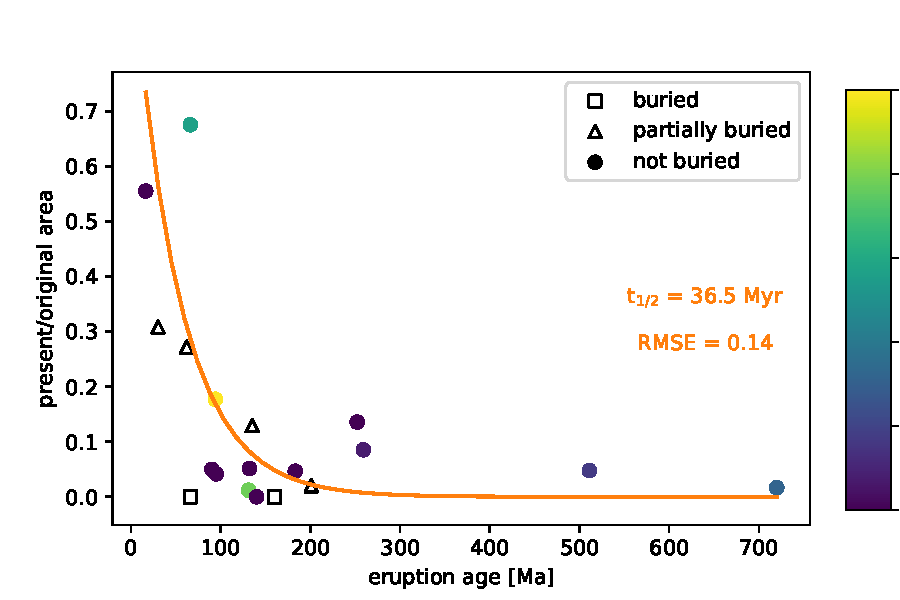
\includegraphics[width=0.65\textwidth]{Manuscript/Figures/LIP_Preservation.pdf}
	\caption{\textbf{LIP preservation through time. The ratio of estimates of the present-day area to that of the original area are shown for 17 basaltic LIPs. The best-fit exponential function to these data is shown which has a half-life of 36 Myr.}}
	\label{fig:LIP_preservation}
\end{center}
\end{figure}

\begin{figure}[h!]
\begin{center}
	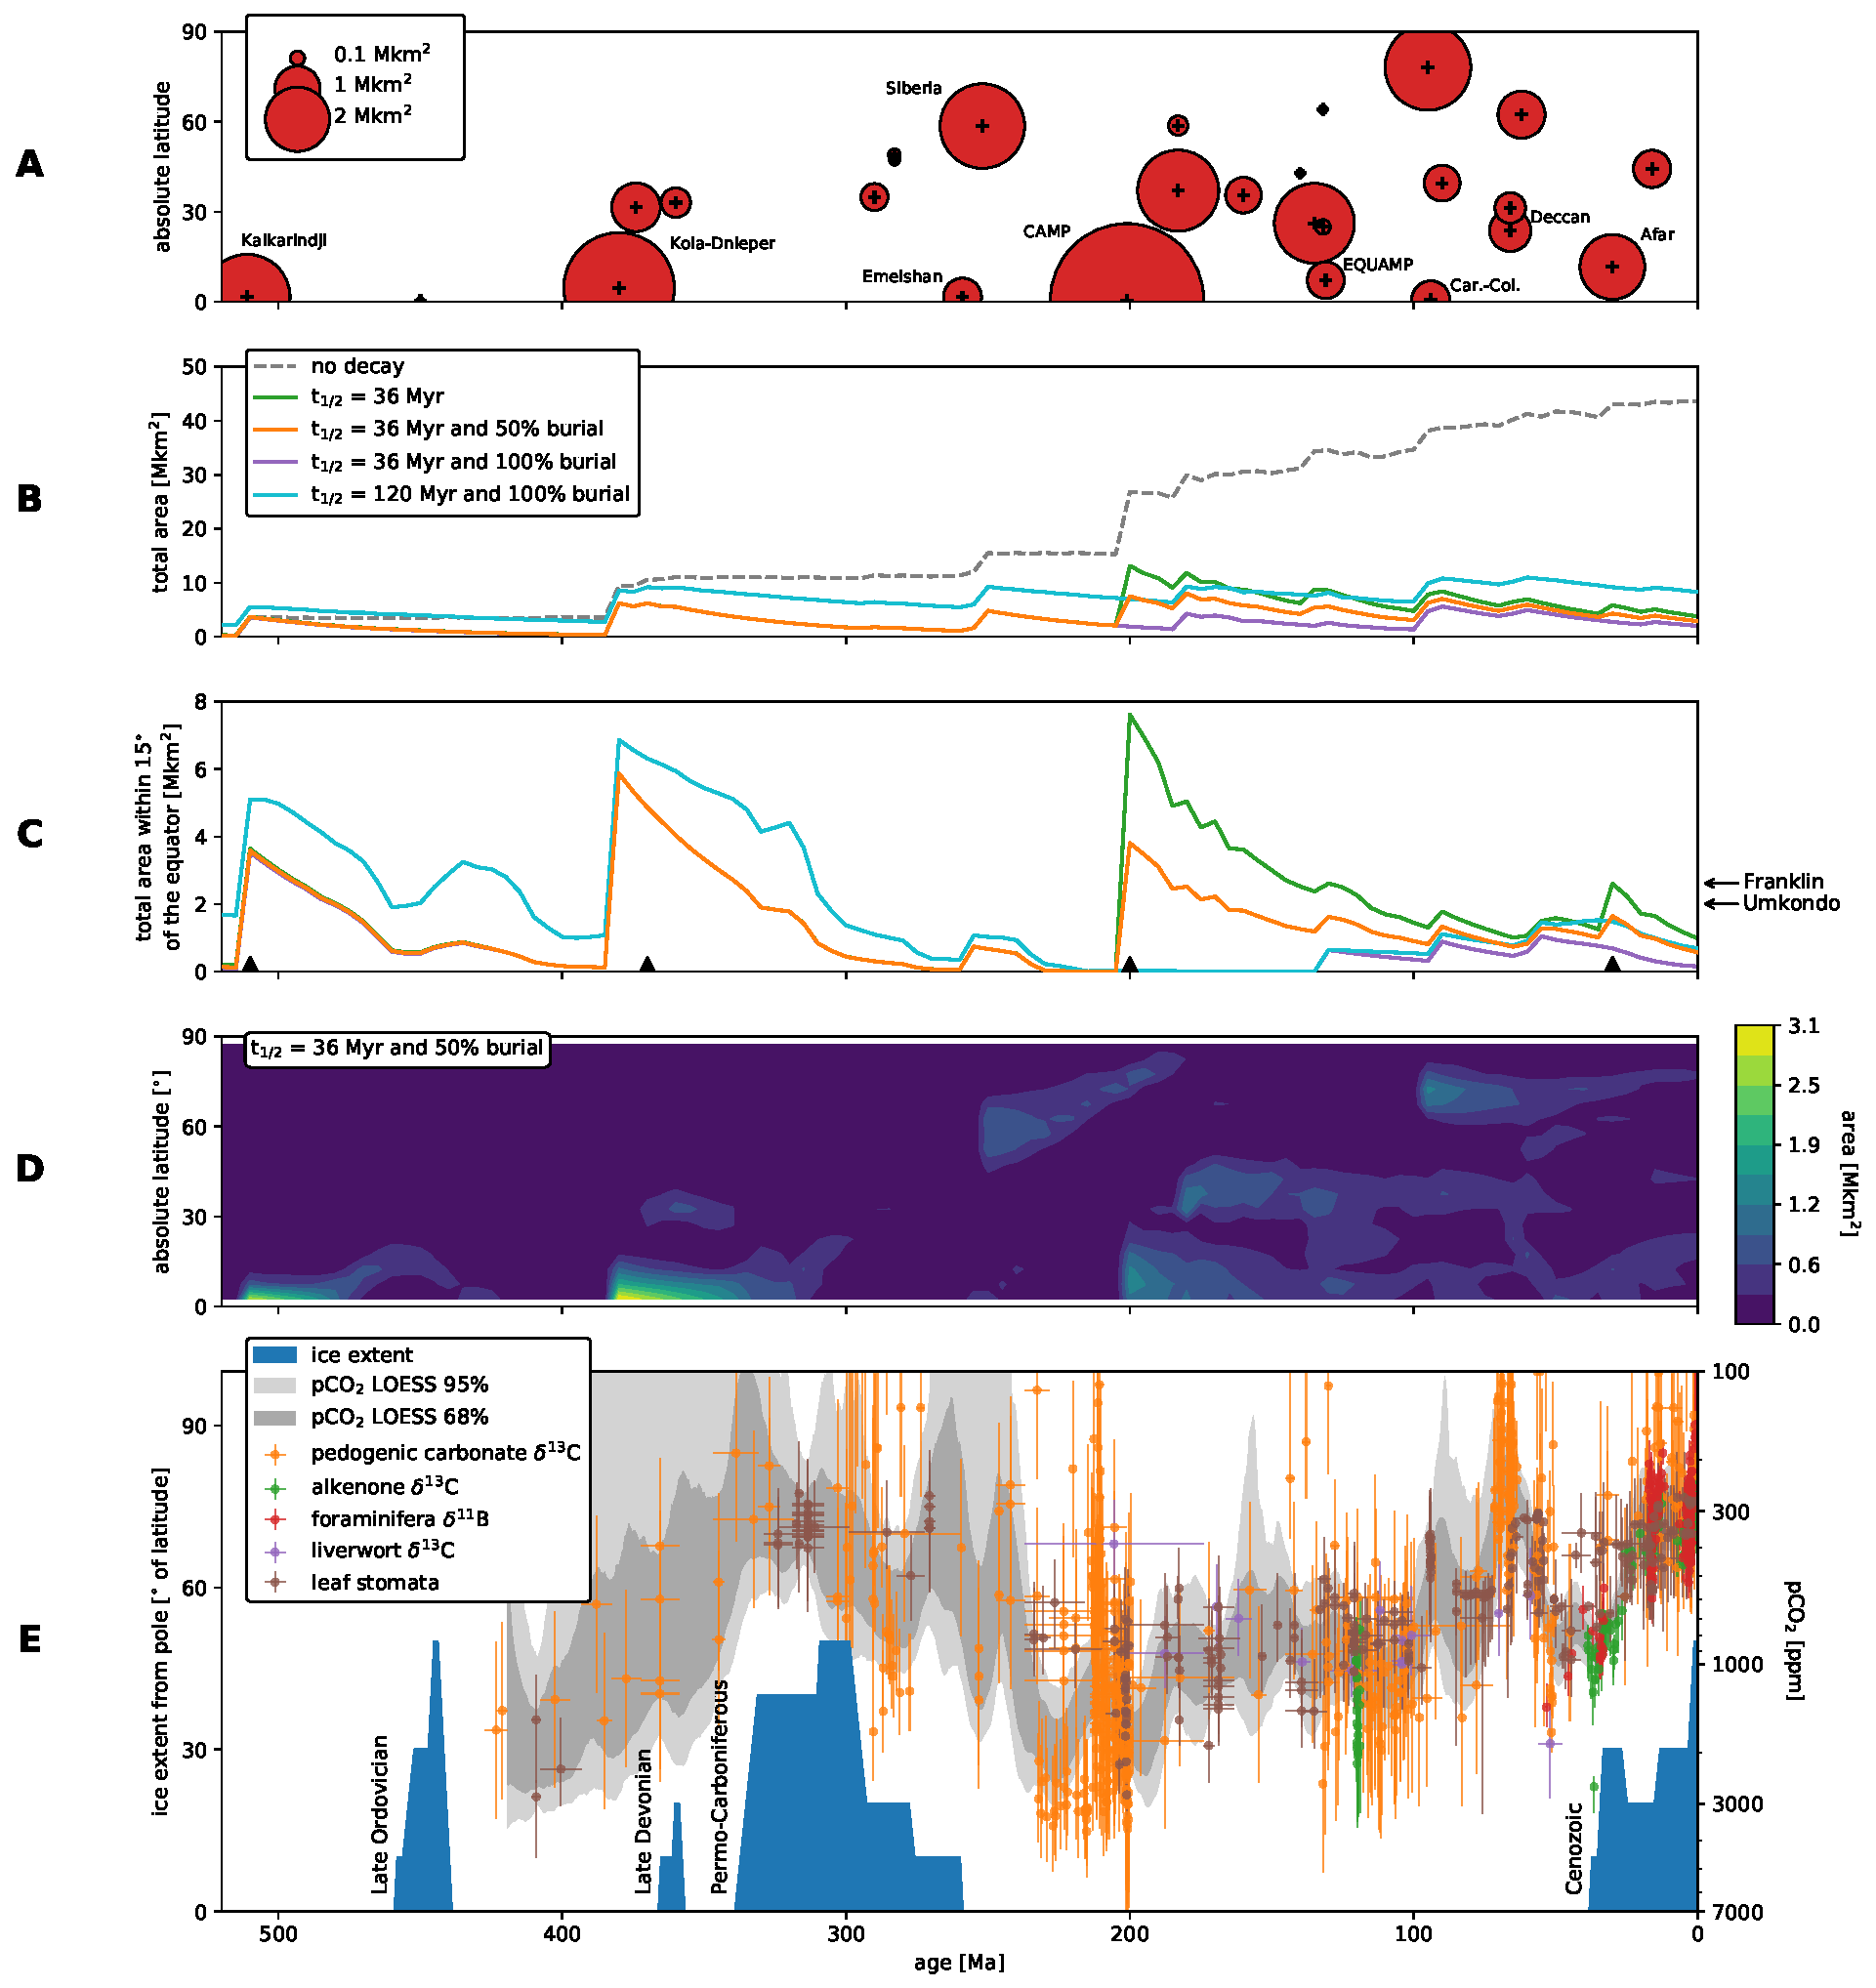
\includegraphics[width=0.9\textwidth]{Manuscript/Figures/LIP_Areas.pdf}
	\caption{\textbf{A) paleolatitude of emplacement and the initial area estimate of each LIP in the compilation.
    B) total LIP area through time for the different post-emplacement models.
    C) tropical LIP area through time for the different post-emplacement models.
    D) heat map for one of the models showing the latitudinal distribution of LIP area.
    E) latitudinal extent away from the poles of land ice through time.}}
	\label{fig:LIP_area}
\end{center}
\end{figure}

\begin{figure}[h!]
\begin{center}
	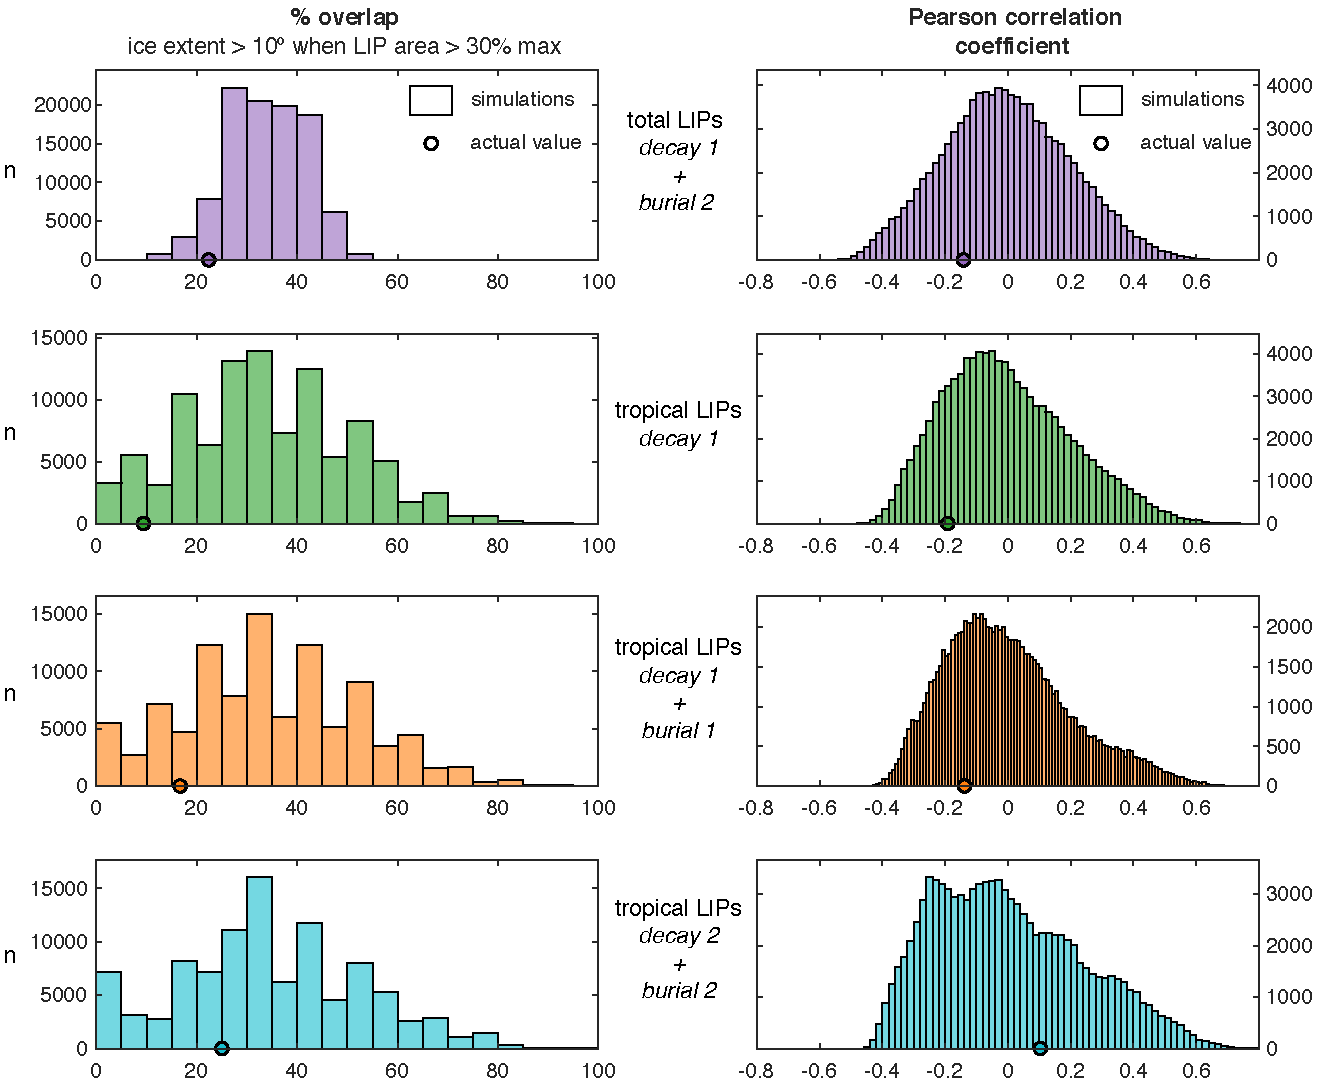
\includegraphics[width=0.85\textwidth]{Manuscript/Figures/overlap_correlation_cropped.pdf}
	\caption{\textbf{The overlap and correlation values for various LIP post-emplacement scenarios are shown with circles (d1 : LIP decay with half-life of 36 Myr; d2: LIP decay with half-life of 120 Myr; b1: 50$\%$ burial of LIPs associated with rifting; b2: 100$\%$ burial of LIPs associated with rifting). These values are compared to histograms that are range of values that arise when comparing the LIP area record to glacial intervals that have been shifted randomly in time 100,000 times. The only scenario for which there is a positive correlation coefficient related to ice extent and LIP area is that of a relatively slow decay rate (d2) and complete burial of LIPs associated with rifting (b2). This positive correlation is weak (\textit{r}=0.10) and is not significant as randomly timed glacial intervals correlate better than the record 28$\%$ of the time. With an associated p-value of 0.28, the null hypothesis that glacial intervals not related to LIP area in the tropics cannot be rejected.}}
	\label{fig:LIP_correlation}
\end{center}
\end{figure}



\clearpage
\newpage
\footnotesize

\singlespacing

\bibliographystyle{gsabull}
\bibliography{References}

\end{document}
